% 运动积分
% 拉格朗日方程|欧拉定理|广义动量|哈密顿量|守恒

\pentry{拉格朗日方程\upref{Lagrng}, 齐次函数的欧拉定理\upref{Homeul}}

我们知道拉格朗日方程是关于广义坐标$q_\alpha(\alpha=1,2,\cdots,s)$的二阶微分方程.在一些情况下,在系统运动过程中,存在$q_\alpha$和$\dot{q}_\alpha$的某些函数,它们不随时间而变,这些函数称为系统的\textbf{运动积分}(integral of motion).运动积分是通常的守恒律,如动量守恒定律、角动量守恒定律、机械能守恒定律的概念的推广.可以看出,运动积分相对于拉格朗日方程而言降了一阶,是一阶的微分方程,所以运动积分有时也称为\textbf{第一次积分}.力学中的对称性是十分重要的,而运动积分的存在与否,与系统的对称性有密切的关系.一个系统如果有尽可能多的运动积分,将对问题的求解带来极大的方便.

\subsection{可遗坐标与广义动量积分}

若拉格朗日函数$L$不含某个广义坐标$q_\beta$,即$\dfrac{\partial L}{\partial q_\beta}=0$,则这种广义坐标叫做\textbf{可遗坐标(ignorable coordinates)}, 也称为\textbf{循环坐标(cyclic coordinates)}. 于是, 拉格朗日方程写为
\begin{equation}
\frac{\mathrm{d}}{\mathrm{d} t}\left(\frac{\partial L}{\partial \dot{q}_{\beta}}\right)=0
\end{equation}
这是说,广义动量$p_\beta=\dfrac{\partial L} {\partial \dot{q_\beta}}$是守恒的,
\begin{equation}
p_\beta=常数(如L不含有q_\beta)
\end{equation}
这叫做\textbf{广义动量积分}.

我们知道,若循环坐标$q_\beta$是系统的整体平移坐标,即拉格朗日函数$L $对于整体平移是不变的,可知广义动量积分归结为动量守恒定律.若拉格朗日函数不包含整体转动坐标,即拉格朗日函数$L$对于整体转动是不变的(各向同性),则广义动量积分归结为角动量守恒定律.

在矢量力学中,动量守恒定律和角动量守恒定律是以牛顿第三定律为先决条件,即内力的矢量和为零、内力的力矩和为零,而\textbf{广义动量积分则并不以牛顿第三定律为先决条件}.这点在后续讨论电磁场时十分明显,很难根据电磁场与粒子的相互作用来谈牛顿第三定律.

\begin{example}{两个楔子的加速度}
质量为$M $的光滑大楔子置于光滑的水平桌面上,质量为$m$的光滑小楔子沿着大楔子的光滑斜边滑下,如\autoref{motint_fig1} 所示.求这两个楔子的加速度.
\begin{figure}[ht]
\centering
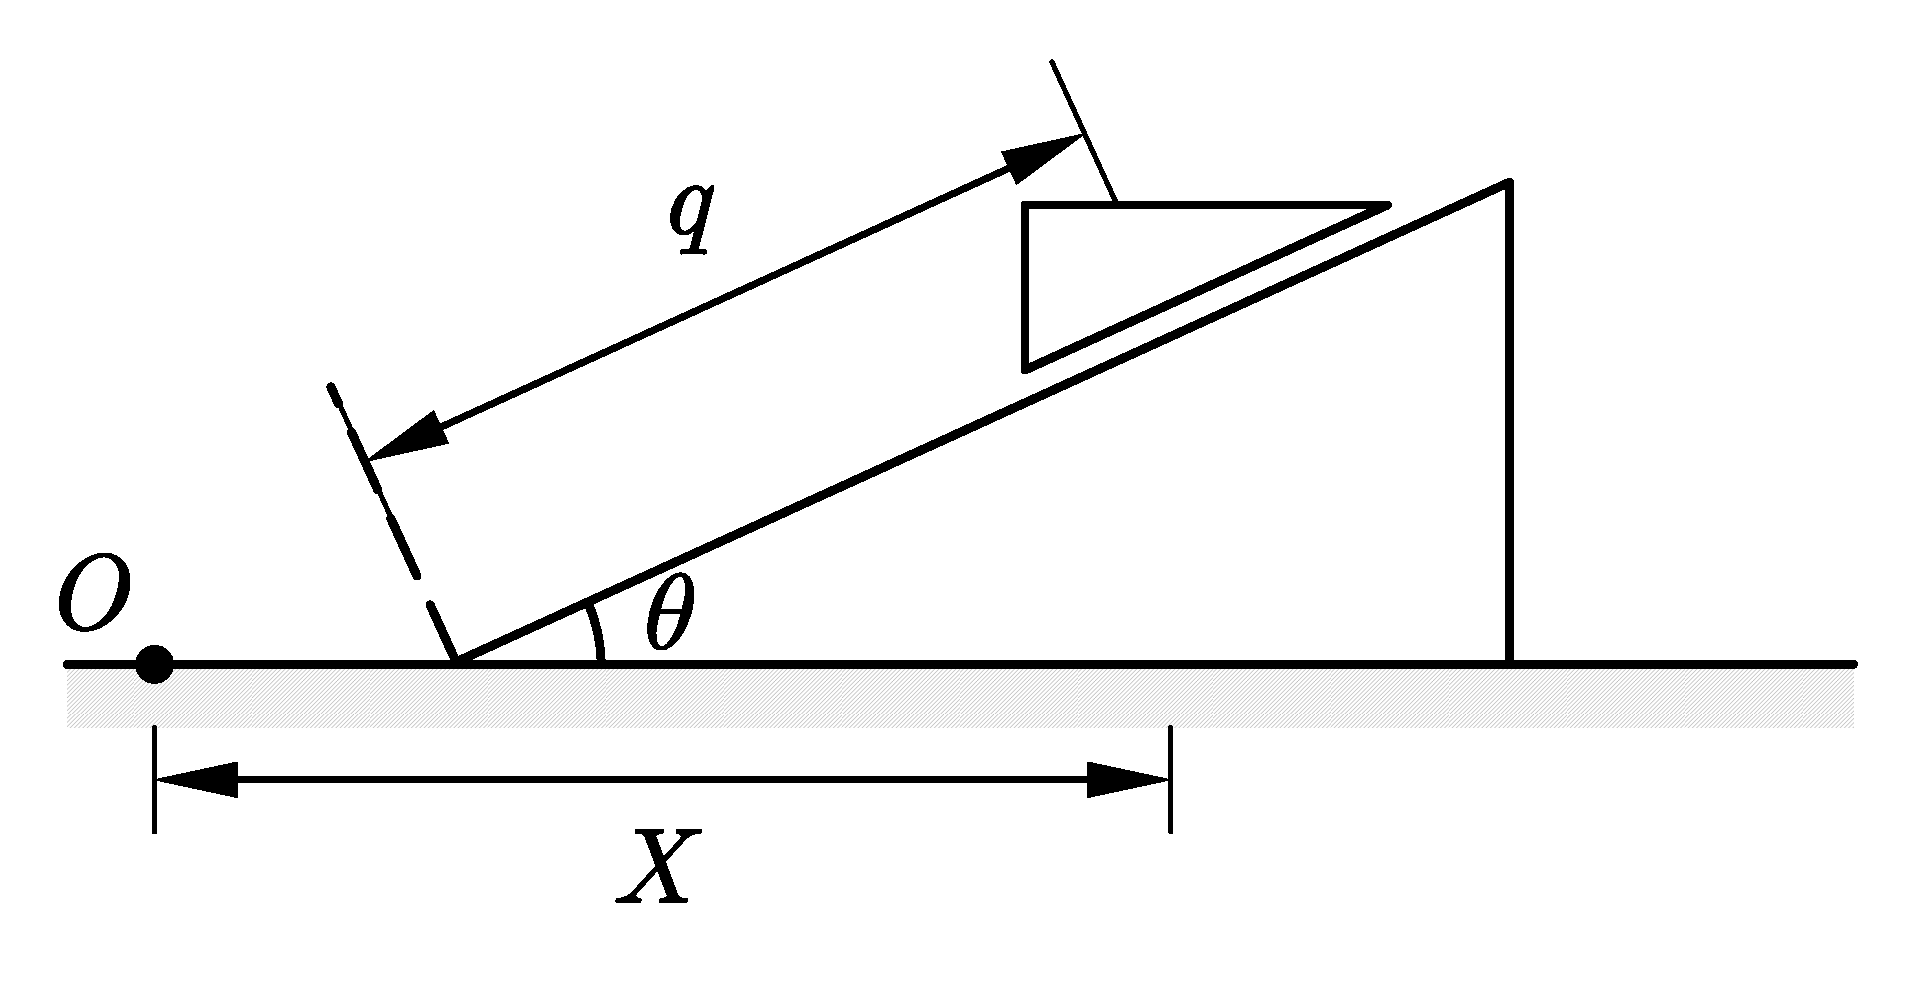
\includegraphics[width=7.5cm]{./figures/motint_1.pdf}
\caption{两个楔子} \label{motint_fig1}
\end{figure}

解:大楔子可在水平方向运动,小楔子在大楔子斜边上运动系统有两个自由度.

取桌面上的固定点$O$,把大楔子的质心相对于$O$点的水平坐标记作$X $.把小楔子的质心相对于大楔子斜边底端、沿着斜边计算的坐标记作$q$(其实取的时候不需要一定是质心,物体上的任一点都可以).这个系统的广义坐标就是$X $和$q $.

主动力是两个楔子所受的重力,它们都是势力.大楔子的势能在运动过程中不变,不需要考虑,只需要讨论小楔子的势能.计算动能需注意,小楔子的速度不仅仅是沿斜边的$\dot q$,而且还有随着大楔子在水平方向运动的速度$\dot X$.可得:
\begin{equation}
\begin{aligned} T &=\frac{1}{2} M \dot{X}^{2}+\frac{1}{2} m\left[v_{\text {水平 }}^{2}+v_{\text {竖直 }}^{2}\right] \\ &=\frac{1}{2} M \dot{X}^{2}+\frac{1}{2} m\left[(\dot{X}+\dot{q} \cos \theta)^{2}+\dot{q}^{2} \sin ^{2} \theta\right] \\ V &=m g q \sin \theta \\ L &=T-V=\frac{1}{2}(M+m) \dot{X}^{2}+\frac{1}{2} m \dot{q}^{2}+m \dot{X} \dot{q} \cos \theta-m g q \sin \theta \end{aligned}
\end{equation}

由拉格朗日方程
\begin{equation}
\begin{cases}
\dfrac{\mathrm{d}}{\mathrm{d} t}[M \dot{X}+m(\dot{X}+\dot{q} \cos \theta)]=0 \\ \dfrac{\mathrm{d}}{\mathrm{d} t}[m(\dot{X} \cos \theta+\dot{q})]+m g \sin \theta=0
\end{cases}
\end{equation}

第一个方程指出,这个系统在水平方向的动量守恒.事实上,$X$是可遗坐标,所以相应的广义动量守恒.

由运动方程解得大楔子的加速度
\begin{equation}
\ddot{X}=\frac{m g \sin \theta \cos \theta}{M+m \sin ^{2} \theta}
\end{equation}
以及小楔子相对于大楔子的加速度
\begin{equation}
\ddot{q}=-\frac{(M+m) g \sin \theta}{M+m \sin ^{2} \theta}
\end{equation}
\end{example}
从此例题可以再次看出用拉格朗日方法解题的优越性.

\subsection{广义能量积分}

拉格朗日函数$L $是时间$t$ 、广义坐标$q $和广义速度$\dot q$的函数.$ L $的时间变化率
\begin{equation}
\frac{\mathrm{d} L}{\mathrm{d} t}=\frac{\partial L}{\partial t}+\sum_{\alpha=1}^{s} \frac{\partial L}{\partial q_{\alpha}} \dot{q}_{\alpha}+\sum_{\alpha=1}^{s} \frac{\partial L}{\partial \dot{q}_{\alpha}} \frac{\mathrm{d} \dot{q}_{\alpha}}{\mathrm{d} t}
\end{equation}
在主动力全是保守力的情况下,利用完整系统的拉格朗日方程,把$\dfrac{\partial L}{\partial q_{\alpha}}$改写,得
\begin{equation}
\begin{aligned} \frac{\mathrm{d} L}{\mathrm{d} t} &=\frac{\partial L}{\partial t}+\sum_{\alpha=1}^{s} \frac{\mathrm{d}}{\mathrm{d} t}\left(\frac{\partial L}{\partial \dot{q}_{\alpha}}\right) \dot{q}_{\alpha}+\sum_{\alpha=1}^{s} \frac{\partial L}{\partial \dot{q}_{\alpha}} \frac{\mathrm{d} \dot{q}_{\alpha}}{\mathrm{d} t} \\ &=\frac{\partial L}{\partial t}+\frac{\mathrm{d}}{d t}\left(\sum_{\alpha=1}^{s} \frac{\partial L}{\partial \dot{q}_{\alpha}} \dot{q}_{\alpha}\right) \end{aligned}
\end{equation}
$\dfrac{\partial L}{\partial \dot{q}_{\alpha}}$就是广义动量$p_\alpha$,这样
\begin{equation} \label{motint_eq1}
\frac{\mathrm{d}}{\mathrm{d} t}\left(\sum_{\alpha=1}^{s} p_{\alpha} \dot{q}_{\alpha}-L\right)=-\frac{\partial L}{\partial t}
\end{equation}
定义\textbf{广义能量函数}(其实就是哈密顿量\upref{HamCan})
\begin{equation} \label{motint_eq2}
H=\sum_{\alpha=1}^{s} p_{\alpha} \dot{q}_{\alpha}-L=\sum_{\alpha=1}^{s} \frac{\partial L}{\partial \dot{q}_{\alpha}} \dot{q}_{\alpha}-L
\end{equation}
则式子\autoref{motint_eq1} 可以写为
\begin{equation}
\frac{\mathrm{d} H}{\mathrm{d} t}=-\frac{\partial L}{\partial t}
\end{equation}
若拉格朗日函数$L$不是时间的显函数,$ L = L(q, \dot q)$, 即
\begin{equation}
\frac{\partial L}{\partial t}=0
\end{equation}
则有\textbf{广义能量积分}(或称\textbf{雅可比积分}).

我们需要清楚广义能量函数的意义.首先,势能$V$是与广义速度无关的,因此$H$的定义\autoref{motint_eq2} 中的$\dfrac{\partial L}{\partial \dot q_\alpha}$.可代之以$\dfrac{\partial T}{\partial \dot q_\alpha}$.

设变换式$\bvec{r}_{i}=\bvec{r}_{i}(q)$不显含时间,即$\partial \bvec{r}_{i} / \partial t=0$, 则
\begin{equation}
\dot{\bvec{r}}_{i}=\sum_{\alpha=1}^{s} \frac{\partial \bvec{r}_{i}}{\partial q_{\alpha}} \dot{q}_{\alpha}
\end{equation}
于是
\begin{equation}
\begin{aligned} T &=\sum_{i=1}^{n} \frac{1}{2} m_{i} \dot{\bvec{r}}_{i} \cdot \dot{\bvec{r}}_{i}=\sum_{i=1}^{n} \frac{1}{2} m_{i} \sum_{\alpha=1}^{s} \dot{q}_{\alpha} \frac{\partial \bvec{r}_{i}}{\partial q_{\alpha}} \cdot \sum_{\beta=1}^{s} \frac{\partial \bvec{r}_{i}}{\partial q_{\beta}} \dot{q}_{\beta} \\ &=\sum_{i=1}^{n} \sum_{\alpha=1}^{s} \sum_{\beta=1}^{s} \frac{1}{2} m_{i} \frac{\partial \bvec{r}_{i}}{\partial q_{\alpha}} \cdot \frac{\partial \bvec{r}_{i}}{\partial q_{\beta}} \dot{q}_{\alpha} \dot{q}_{\beta} \end{aligned}
\end{equation}
这是广义速度的二次齐次多项式.根据齐次函数的欧拉定理,有
\begin{equation} \label{motint_eq3}
\sum_{\alpha=1}^{s} \frac{\partial T}{\partial \dot{q}_{\alpha}} \dot{q}_{\alpha}=2 T
\end{equation}
其实这也可以直接验证:
\begin{equation}
\begin{aligned} \frac{\partial T}{\partial \dot{q}_{\gamma}} &=\sum_{i=1}^{n} \sum_{\alpha=1}^{s} \frac{1}{2} m_{i} \frac{\partial \bvec{r}_{i}}{\partial q_{\alpha}} \cdot \frac{\partial \bvec{r}_{i}}{\partial q_{\gamma}} \dot{q}_{\alpha}+\sum_{i=1}^{n} \sum_{\beta=1}^{s} \frac{1}{2} m_{i} \frac{\partial \bvec{r}_{i}}{\partial q_{\gamma}} \cdot \frac{\partial \bvec{r}_{i}}{\partial q_{\beta}} \dot{q}_{\beta} \\ &=\sum_{i=1}^{n} \sum_{\alpha=1}^{s} m_{i} \frac{\partial \bvec{r}_{i}}{\partial q_{\alpha}} \cdot \frac{\partial \bvec{r}_{i}}{\partial q_{\gamma}} \dot{q}_{\alpha} \end{aligned}
\end{equation}
于是
\begin{equation}
\sum_{\gamma=1}^{s} \frac{\partial T}{\partial \dot{q}_{\gamma}} \dot{q}_{\gamma}=\sum_{i=1}^{n} \sum_{\alpha=1}^{s} \sum_{\gamma=1}^{s} m_{i} \frac{\partial \bvec{r}_{i}}{\partial q_{\alpha}} \cdot \frac{\partial \bvec{r}_{i}}{\partial q_{\gamma}} \dot{q}_{\alpha} \dot{q}_{\gamma}=2 T
\end{equation}

由此,广义能量函数
\begin{equation}
H=\sum_{\alpha=1}^{s} p_{\alpha} \dot{q}_{\alpha}-L=2 T-(T-V)=T+V
\end{equation}
这样,在变换式$\bvec{r}_{i}=\bvec{r}_{i}(q)$不显含时间的条件下,动能是广义速度的二次齐次式,广义能量函数$H $就是机械能.如果约束是非定常的,则变换式$\bvec{r}_{i}=\bvec{r}_{i}(q, t)$难免显含时间.即使约束是稳定的,也可能由于选择了某些广义坐标(例如平移坐标系),变换式$\bvec{r}_{i}=\bvec{r}_{i}(q, t)$显含时间$t $.在变换式显含时间的情况下,
\begin{equation}
\dot{\bvec r}_{i}=\frac{\partial \bvec{r}_{i}}{\partial t}+\sum_{\alpha=1}^{s} \frac{\partial \bvec{r}_{i}}{\partial q_{\alpha}} \dot{q}_{\alpha}
\end{equation}
于是
\begin{equation}
\begin{aligned} T=& \sum_{i=1}^{n} \frac{1}{2} m_{i}\left(\frac{\partial \bvec{r}_{i}}{\partial t}+\sum_{\alpha=1}^{s} \frac{\partial \bvec{r}_{i}}{\partial q_{\alpha}} \dot{q}_{\alpha}\right) \cdot\left(\frac{\partial \bvec{r}_{i}}{\partial t}+\sum_{\beta=1}^{s} \frac{\partial \bvec{r}_{i}}{\partial q_{\beta}} \dot{q}_{\beta}\right) \\=& \sum_{i=1}^{n}\left\{\frac{1}{2} m_{i}\left(\frac{\partial \bvec{r}_{i}}{\partial t}\right)^{2}+\sum_{\alpha=1}^{s} m_{i} \frac{\partial \bvec{r}_{i}}{\partial t} \cdot \frac{\partial \bvec{r}_{i}}{\partial q_{\alpha}} \dot{q}_{\alpha}\right.\\ &\left.+\sum_{\alpha=1}^{s} \sum_{\beta=1}^{s} \frac{1}{2} m_{i} \frac{\partial \bvec{r}_{i}}{\partial q_{\alpha}} \cdot \frac{\partial \bvec{r}_{i}}{\partial q_{\beta}} \dot{q}_{\alpha} \dot{q}_{\beta}\right\} \end{aligned}
\end{equation}
这包含三个部分,它们分别是广义速度的零次、一次、二次的齐次多项式,分别记作$T_0,T_1,T_2$,即$T=T_0+T_1+T_2$.根据齐次函数的欧拉定理,
\begin{equation}
\sum_{\alpha=1}^{s} \frac{\partial T}{\partial \dot{q}_{\alpha}} \dot{q}_{\alpha}=0 T_{0}+1 T_{1}+2 T_{2}=T_{1}+2 T_{2}
\end{equation}
由此,广义能量函数
\begin{equation}
H=\sum_{\alpha=1}^{s} p_{\alpha} \dot{q}_{\alpha}-L=\left(T_{1}+2 T_{2}\right)-\left(T_{0}+T_{1}+T_{2}-V\right)=T_{2}-T_{0}+V
\end{equation}

这样,在变换式显含时间的条件下,广义能量函数$H $并非机械能,但是具有机械能的量纲,故名之为\textbf{广义能量}.

\begin{example}{直线运动汽车里的谐振子}
在匀速直线运动的汽车中,有一谐振子在光滑水平槽中往返振动.取沿振动方向的坐标为$q$,原点在谐振子的平衡点.选汽车为参考系,于是它是惯性系.谐振子的拉格朗日函数$L=T-V=m \dot{q}^{2} / 2-k q^{2} / 2$.易见$\partial L / \partial t=0$,所以$H $守恒.另一方面,由于动能$T=m \dot{q}^{2} / 2$是广义速度$\dot q $的二次单项式,所以$H $就是机械能.诚然,$ H=p\dot q-L=(\partial L / \partial \dot{q}) \dot{q}-L=m \dot{q}^{2} / 2+k q^{2} / 2=T+V$.

改取地面为参考系,这也可认为是惯性系.如果谐振子的振动方向平行于汽车运动方向,则谐振子的$L=T-V=m\left(\dot{q}+v_{0}\right)^{2} / 2-k q^{2} / 2=m \dot{q}^{2} / 2+m v_{0} \dot{q}+m v_{0}^{2} / 2-k q^{2} / 2$,其中$v_0$是汽车的速度.因$\partial L / \partial t=0$, 所以$H $守恒.但动能$T$不是$\dot q $的二次齐次式,所以$H $并非机械能.实际上我们可以通过写出$H$的表达式来说明这一点:$H=p \dot{q}-L=m\left(\dot{q}+v_{0}\right) \dot{q}-L=m \dot{q}^{2} / 2-m v_{0}^{2} / 2+k q^{2} / 2 \neq T+V$.

如果汽车并非匀速,我们考察它的匀加速运动,即速度为$at $.仍以地面为参考系,则谐振子的$m(\dot{q}+a t)^{2} / 2-k q^{2} / 2$,这时$\partial L / \partial t \neq 0$, 所以$H $不守恒.另一方面,$T$不是$\dot q $的二次齐次式,所以$H$也不是机械能.实际上,$H=m \dot{q}^{2} / 2-m a^{2} t^{2} / 2+k q^{2} / 2 \neq T+V$.
\end{example}
